\chapter{Particle--mesh gravity, time stepping and COLA}\label{ch:nbody-pm}
\chapterstatus{written}{2026-11-26}

This chapter describes how \fml{} moves particles under their own gravity: the comoving equations of motion and their
units, the particle--mesh (PM) force with its choices of Green's function, gradient, assignment and anti-aliasing,
the four time integrators (Quinn, Tassev, FastPM and BullFrog), including velocity friction and several species, and
the COLA method, in its scale-independent and scale-dependent forms. Short-range corrections to the PM force are in
\cref{ch:short-range}; the complete simulation program in \cref{ch:simulation-code}.

\begin{modulebox}{NBody}
\file{NBody/NBody.h} (namespace \nsp{FML::NBODY}): density assignment, Poisson solve, forces, kick and drift;
\file{NBody/ForceOptions.h} (\cls{ForceOptions}); \file{NBody/TimeStepping.h}, \file{NBody/TimeStepTypes.h}
(\cls{TimeStepping}, \cls{TimestepOptions}); \file{LPT/GrowthHistory.h}.\par
SimulationCode: \file{src/KickDrift.h}, \file{src/COLA.h}, \file{src/SimulationStep.h}, \file{src/SpeciesTimeStepping.h},
\file{src/TimeStepping.h}.\par
Documentation: \file{NBody/ForceOptions.md}, \file{NBody/TimeStepping.md}, \file{SimulationCode/EVOLUTION.md},
\file{SimulationCode/DYNAMICS.md}.
\end{modulebox}

\section{Equations of motion}\label{sec:nbody-eom}

Particles move in comoving coordinates $\vx$, in units of the box size $B$. With the canonical code velocity
\begin{equation}
\bm v\equiv a^3E(a)\frac{\dd\vx}{\dd a}=\frac{a^2}{H_0}\frac{\dd\vx}{\dd t},
\end{equation}
the equations of motion of a cold particle are
\begin{equation}
\frac{\dd\vx}{\dd a}=\frac{\bm v}{a^3E(a)},\qquad \frac{\dd\bm v}{\dd a}=-\frac{\nabla\phi}{a^3E(a)},\qquad
\nabla^2\phi=\frac32\Om_m\,a\,\mu(k,a)\,\delta,
\label{eq:nbody-eom}
\end{equation}
where $\phi$ is the peculiar potential in units of $(H_0B)^2$ and $\nabla$ is with respect to $\vx$ in box units. The
\emph{force prefactor} $C(a)=\frac32\Om_ma\,\mu$ carries the time dependence of the force; in GR $\mu=1$. A velocity
friction $\Gamma(a)$, $\dd\bm v/\dd\ln a=-\Gamma\bm v+\ldots$ (dark scattering, coupled quintessence), is optional.

\section{The particle--mesh force}\label{sec:nbody-pm}

A PM step computes $\delta$ on a grid of $N_{\rm mesh}^3$ cells (\param{force_nmesh}), solves the Poisson equation in
Fourier space and interpolates the force back to the particles:
\begin{equation}
\bm F(\vk)=-i\bm D(\vk)\,G(\vk)\,C(a)\,\frac{\delta(\vk)}{W^{2}(\vk)}\quad(\text{deconvolved}),\qquad
\bm F_p=\sum_{\rm cells}W(\vx_p-\vx_{\rm cell})\bm F(\vx_{\rm cell}),
\end{equation}
with the assignment window $W$ of order $p$ (NGP, CIC, TSC, PCS, PQS; \cref{ch:mass-assignment}),
$W(\vk)=\prod_j[\mathrm{sinc}(k_j\Delta x/2)]^p$, used both to assign and to interpolate so that the self-force vanishes
and momentum is conserved \cite{HockneyEastwood1988}. In SimulationCode the kernel is \param{force_density_assignment_method}
(CIC by default) and \param{force_interpolation_method} chooses how the force reaches the particles: with the same kernel
(\code{assignment}), or by evaluating its Fourier series exactly at the particles (\code{nufft}; \code{fiducial}, the
default, does this when the density is also a NUFFT, so that there is still no self-force). The Green's function $G$ and the gradient $\bm D$ (\cls{ForceOptions}) are described in \cref{sec:nbody-kernels}. There are no global defaults: each call takes its \cls{ForceOptions}.

\begin{cppcode}[A PM force]
#include <FML/NBody/NBody.h>
FML::NBODY::ForceOptions options;
options.laplace_kernel  = FML::NBODY::DISCRETE_GREENS_FUNCTION_FROM_TWO_POINT;
options.gradient_kernel = FML::NBODY::DISCRETE_FOUR_POINT_GRADIENT;
options.deconvolve      = false;
double norm = 1.5 * OmegaM * a;                       // the Poisson prefactor C(a)
FML::NBODY::compute_force_from_density_fourier<3>(density_fourier, force, "CIC", norm, options);
\end{cppcode}

\subsection{The force kernels}\label{sec:nbody-kernels}

A PM force is built from three kernels: the Green's function $G(\vk)$ that inverts the Laplacian, the gradient
$\bm D(\vk)$ that differentiates the potential ($\nabla\to i\bm D$) and the assignment window $W(\vk)$. With
$\Delta x=1/N_{\rm mesh}$ (box units), $\delta(\vk)$ the Fourier transform of the assigned density and $C$ the Poisson
prefactor ($\nabla^2\Phi=C\delta$), the force on the grid is
\begin{equation}\label{eq:nbody-force-kernels}
\Phi(\vk)=G(\vk)\,C\,\delta(\vk),\qquad
\bm F(\vk)=-i\bm D(\vk)\,\frac{\Phi(\vk)}{W^{n}(\vk)},\qquad
W(\vk)=\prod_{j}\left[\mathrm{sinc}\frac{k_j\Delta x}{2}\right]^{p},
\end{equation}
with $n=0$ (\code{deconvolve = false}, the default) or $n=$ \code{deconvolve_window_power} (2: assignment and
interpolation with the window; 1 if one of them is exact, as with the NUFFT), and $p$ the assignment order
(1 NGP, 2 CIC, 3 TSC, 4 PCS, 5 PQS). The exact force of the band-limited density is $G=-1/k^2$ and $\bm D=\vk$. The
discrete kernels are the Fourier transforms of finite-difference stencils: a stencil acting on $\phi(x_i+l\Delta x)$
becomes a multiplication by $e^{ilk\Delta x}$, so a symmetric difference gives $i\sin$ and a symmetric second difference
$\cos$. All kernels act direction by direction, $\bm D=(D(k_1),D(k_2),D(k_3))$ and
$G=-1/\sum_jL(k_j)$, where $L(k)$ is minus the one-dimensional Laplacian. With $x=k\Delta x$ ($x=\pi$ at the
grid Nyquist frequency $k_{\rm Ny}=\pi/\Delta x$):

\paragraph{Green's functions} (\cls{GreensFunctionLaplaceOperatorKernels}, \param{force_greens_function_kernel};
\code{greens_function_laplace_operator_fourier} in \file{NBody/NBody.h})
\begin{center}\small
\begin{tabularx}{\textwidth}{@{}llXl@{}}
\toprule
Name & Real-space stencil for $\partial^2\phi$ & $L(k)\,\Delta x^2$ & Small $x$ \\
\midrule
\code{continuous} & (spectral) & $x^2$ & exact \\
\code{discrete_2pt} & $\dfrac{\phi_{i+1}-2\phi_i+\phi_{i-1}}{\Delta x^2}$ & $4\sin^2\dfrac{x}{2}=2(1-\cos x)$ & $x^2\left(1-\dfrac{x^2}{12}\right)$ \\[1.5ex]
\code{discrete_4pt} & $\dfrac{-\phi_{i+2}+16\phi_{i+1}-30\phi_i+16\phi_{i-1}-\phi_{i-2}}{12\Delta x^2}$ & $\dfrac{15-16\cos x+\cos 2x}{6}$ & $x^2\left(1-\dfrac{x^4}{90}\right)$ \\
\bottomrule
\end{tabularx}
\end{center}
\code{discrete_2pt} is the 7-point Laplacian in 3D, the discrete Green's function of \citet{HockneyEastwood1988}; it is
second order and makes the potential too large at high $k$ ($L/k^2=0.81$ at $k_{\rm Ny}/2$ and $4/\pi^2=0.41$ at
$k_{\rm Ny}$ along an axis). \code{discrete_4pt} is the fourth-order (5-point per direction) stencil ($L/k^2=0.95$ at
$k_{\rm Ny}/2$, $0.54$ at $k_{\rm Ny}$). Both vanish only at $\vk=0$, where $G$ is set to zero (the mean density does
not source the potential). Until November 2026 \code{discrete_4pt} was $L=D_4^2$, the square of the four-point gradient
below; that vanishes at $k_{\rm Ny}$, so the modes near it got a potential up to $\sim10^4$ times too large and runs
with it blew up. Since the potential is computed once and then differentiated, $G$ and $\bm D$ need not come from the
same stencil: composing the two-point gradient twice gives the wide stencil
$(\phi_{i+2}-2\phi_i+\phi_{i-2})/(4\Delta x^2)$, with $L=\sin^2x/\Delta x^2$, not \code{discrete_2pt}.

\paragraph{Gradients} (\cls{GradientKernels}, \param{force_gradient_kernel}; \code{gradient_kernel_fourier})
\begin{center}\small
\begin{tabularx}{\textwidth}{@{}llXl@{}}
\toprule
Name & Real-space stencil for $\partial\phi$ & $D(k)\,\Delta x$ & Small $x$ \\
\midrule
\code{continuous} & (spectral) & $x$ ($0$ at $x=\pi$) & exact \\
\code{discrete_2pt} & $\dfrac{\phi_{i+1}-\phi_{i-1}}{2\Delta x}$ & $\sin x$ & $x\left(1-\dfrac{x^2}{6}\right)$ \\[1.5ex]
\code{discrete_4pt} & $\dfrac{-\phi_{i+2}+8\phi_{i+1}-8\phi_{i-1}+\phi_{i-2}}{12\Delta x}$ & $\dfrac{8\sin x-\sin 2x}{6}$ & $x\left(1-\dfrac{x^4}{30}\right)$ \\[1.5ex]
6th order (FD only) & $\dfrac{45\delta_1\phi-9\delta_2\phi+\delta_3\phi}{60\Delta x}$, $\delta_l\phi=\phi_{i+l}-\phi_{i-l}$ & $\dfrac{45\sin x-9\sin 2x+\sin 3x}{30}$ & $x\left(1-\dfrac{x^6}{140}\right)$ \\
\bottomrule
\end{tabularx}
\end{center}
$D/k$ is $0.64$, $0.85$ and $0.93$ at $k_{\rm Ny}/2$ for the 2-, 4- and 6-point stencils. Every gradient is zero for the
Nyquist component $k_j=k_{\rm Ny}$ of an even mesh: the discrete ones because $\sin(\pi)=0$, the continuous one by
construction, since that mode is its own mirror image and $ik_j$ would depend on the sign chosen for it (FFTW's
$+k_{\rm Ny}$); with zero there the force of a reflected density is the reflected force. The finite-difference force
(\code{compute_force_from_potential_real}, \param{force_use_finite_difference_force} with
\param{force_finite_difference_stencil_order} $=2,4,6$) applies the stencils in real space to the potential computed
with the chosen Green's function; orders 2 and 4 give the same force as the Fourier gradients \code{discrete_2pt} and
\code{discrete_4pt} (to $10^{-15}$), order 6 exists only there.

\paragraph{The force of a combination.} Without the window, the force of a single mode relative to the exact force
$\vk/k^2$, along the wave vector, is
\begin{equation}
\frac{F_{\rm PM}}{F_{\rm exact}}=\frac{|\vk|\,\hat{\vk}\cdot\bm D(\vk)}{\sum_jL(k_j)}
\;\xrightarrow{\ \vk\parallel\hat{\bm e}_1\ }\;\frac{k\,D(k)}{L(k)} .
\end{equation}
Along an axis, at small $x$, this is $1$ (continuous/continuous), $1-x^2/6$ (two-point $\bm D$, continuous $G$),
$1-x^4/30$ (four-point $\bm D$, continuous or four-point $G$), $1-x^2/12$ (two-point $\bm D$ and $G$) and $1+x^2/12$
(four-point $\bm D$, two-point $G$). The discrete kernels are anisotropic: the same $|\vk|$ along the diagonal
$(1,1,1)/\sqrt3$ has each component $\sqrt3$ times smaller and is closer to exact. \Cref{fig:nbody-force-kernels} shows
the kernels; some values:
\begin{center}\small
\begin{tabular}{@{}llcccc@{}}
\toprule
& & \multicolumn{2}{c}{along an axis} & \multicolumn{2}{c}{along the diagonal} \\
$\bm D$ & $G$ & $k_{\rm Ny}/4$ & $k_{\rm Ny}/2$ & $k_{\rm Ny}/4$ & $k_{\rm Ny}/2$ \\
\midrule
continuous & continuous & 1 & 1 & 1 & 1 \\
\code{discrete_2pt} & continuous & 0.900 & 0.637 & 0.966 & 0.869 \\
\code{discrete_4pt} & continuous & 0.988 & 0.849 & 0.999 & 0.980 \\
\code{discrete_2pt} & \code{discrete_2pt} & 0.948 & 0.785 & 0.983 & 0.931 \\
\code{discrete_4pt} & \code{discrete_2pt} & 1.041 & 1.047 & 1.016 & 1.050 \\
\code{discrete_4pt} & \code{discrete_4pt} & 0.992 & 0.898 & 0.999 & 0.986 \\
continuous & \code{discrete_2pt} & 1.053 & 1.234 & 1.017 & 1.072 \\
\bottomrule
\end{tabular}
\end{center}
Pairing a discrete Green's function with the continuous gradient boosts the force at high $k$ (the potential is too
large and nothing compensates). These are the kernels alone: the window then multiplies the force by $W^{2-n}$ (CIC:
$W^2=0.66$ along an axis at $k_{\rm Ny}/2$), and the aliased images of the assignment add to it, which interlacing
(\param{force_interlacing_order}) reduces: the force is averaged over $M$ copies of the particles shifted by fractions of
a cell, and for the half-cell diagonal ($M=2$) the images at $\vk+2k_{\rm Ny}\bm n$ with odd $\sum_jn_j$ get the
phase $-1$ and cancel. On a grid finer than the particle grid the kernels also decide how the lattice signal at the
grid Nyquist frequency reaches the particles (next subsection), which is why SimulationCode's fiducial gradient is not
the continuous one there.

\begin{figure}[htbp]
\centering
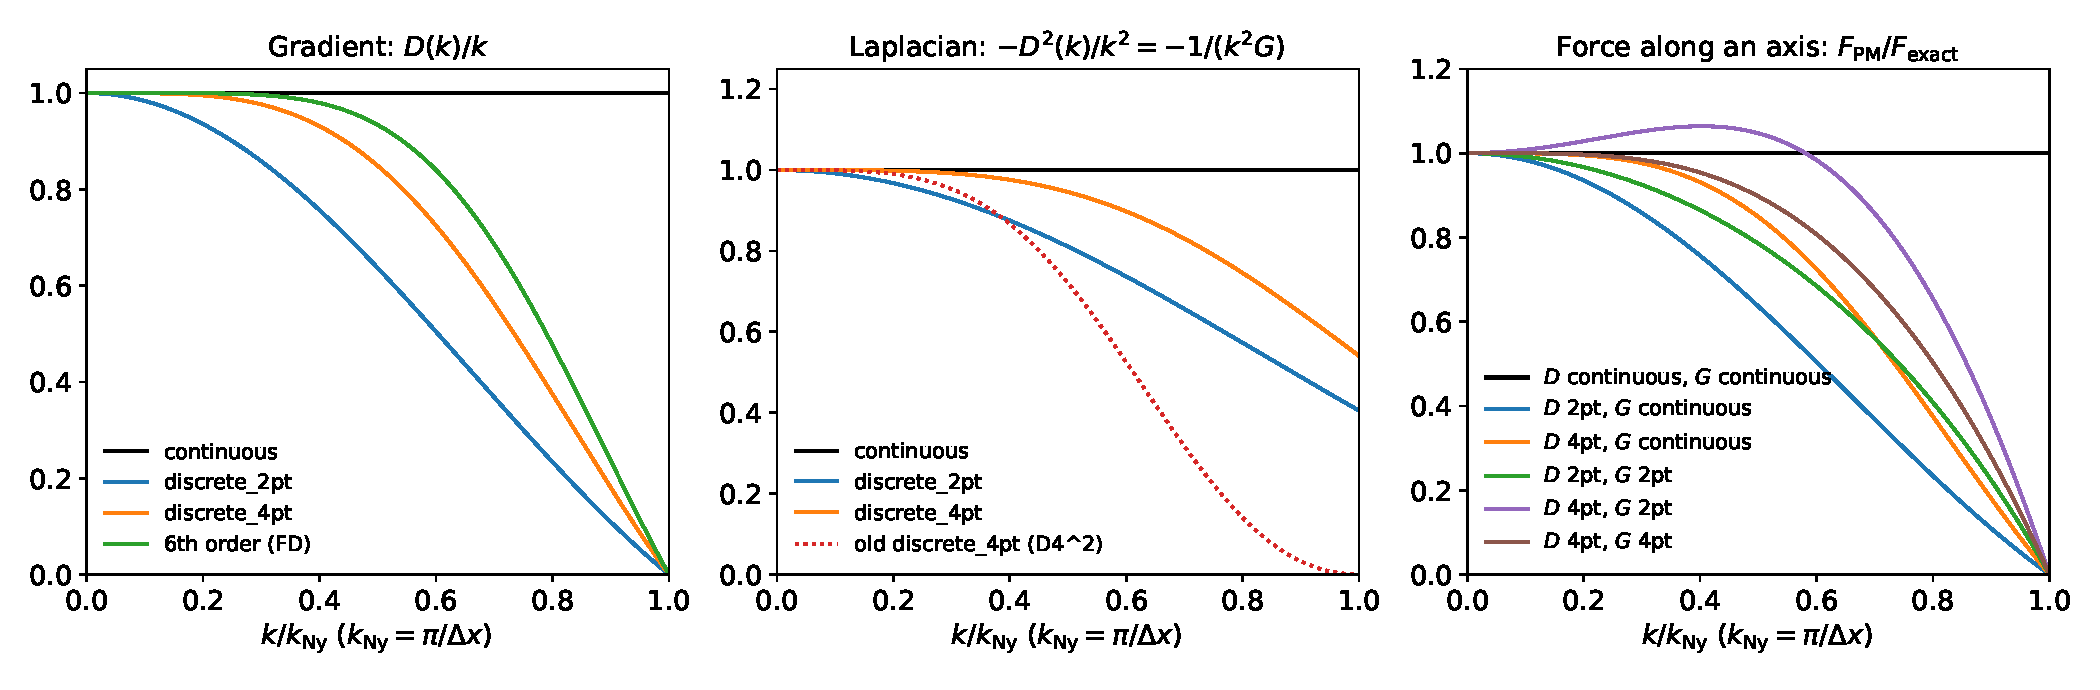
\includegraphics[width=\textwidth]{force_kernels}
\caption{The force kernels of \cls{ForceOptions} along a grid axis: the gradients $D(k)/k$ (\emph{left}; the sixth order
is the finite-difference force), the Laplacians $L(k)/k^2=-1/(k^2G)$ (\emph{middle}; dotted: the pre-November 2026
\code{discrete_4pt}, $D_4^2$, which vanishes at $k_{\rm Ny}$) and the force of the combinations relative to the exact
force, without the assignment window (\emph{right}). Made with \file{Documentation/tools/force_kernels_figure.py}.}
\label{fig:nbody-force-kernels}
\end{figure}

\paragraph{Choosing.} The library default (an omitted \cls{ForceOptions}) is continuous $G$ and $\bm D$ without
deconvolution. SimulationCode's \code{fiducial} is the continuous Green's function and, for the gradient, continuous
for $N_{\rm mesh}=N_p^{1/3}$, \code{discrete_4pt} for $N_p^{1/3}<N_{\rm mesh}\le3N_p^{1/3}$ and \code{discrete_2pt} for
finer grids, with the lattice offset by half a force cell. In the PM settings study ($64^3$ particles in
$250\Mpch$) \code{discrete_4pt} for $G$ gives $P(k)$ within $0.1\%$ of the continuous $G$ to
$k=0.3\hMpc$ and \code{discrete_2pt} $+8.5\%$; the larger effects come from the grid size and the window
(\cref{sec:nbody-pm}, \file{SimulationCode/tests/check_pm_settings.py}).

\begin{validation}[Validation: force kernels (\file{tests/test_nbody.cpp})]
\code{test_nbody} checks the \code{discrete_4pt} Green's function against its 5-point stencil (to $10^{-15}$) and that it is bounded at the Nyquist frequency ($k^2|G|\le1.85$), the plane-wave force $\sin(kx)\,D_4/L_4$ of the four-point kernels, that the force of a reflected density is the reflected force also for the Nyquist modes (which needs the zero Nyquist gradient), and that the finite-difference force equals the Fourier force of the same stencil, with and without deconvolution.
\code{check_pm_settings.py} (1--3 minutes) runs a $64^3$ simulation with each setting, \code{discrete_4pt} $G$
included, against a converged run.
\end{validation}

\subsection{The force grid, the lattice and the gradient kernel}

COLA and PM runs usually use a force grid 2--4 times finer than the particle grid. With an integer ratio
$m=N_{\rm mesh}/N_p^{1/3}$ the particles of a lattice start exactly on grid nodes, where the CIC kernel has a kink, so
the assigned density responds to the \emph{size} of the displacement: a rectified signal at the lattice frequency
(the grid Nyquist frequency for $m=2$). With the continuous gradient, which is large near Nyquist, this gives spurious
forces (the growth of single large-scale modes off by tens of per cent). SimulationCode's fiducial settings therefore
offset the lattice by half a force cell (\param{ic_lattice_offset}) and use the four-point gradient for grids up to
$3\times$ the particle grid and the two-point gradient for finer grids (\param{force_gradient_kernel}
\code{= fiducial}). With these, $P(k)$ at $z=0$ agrees with a $6\times$ TSC reference to $\lesssim1\%$ for $k\le0.4\hMpc$
on 2--4$\times$ grids, against $+10$--$14\%$ for the continuous kernel on a $2\times$ grid with particles on the nodes.

The plain library functions have no such defaults: \code{NBodyInitialConditions} puts the particles on the nodes and
an omitted \cls{ForceOptions} means the continuous gradient. In a linear test ($64^3$ particles, $N_{\rm mesh}=128$,
CIC, displacements much smaller than a cell) the growth of the first six modes is off by factors $0.5$--$3.8$; the
two-point gradient alone brings it to within $1\%$, the four-point gradient to within $9\%$ and TSC to within $4\%$,
while shifting the lattice with the continuous gradient still leaves $+5$--$24\%$. With realistic amplitudes the
particles leave the nodes early and the effect is smaller (in the \file{NBody/example} run the continuous gradient
gives $3$--$6\%$ more power at $k<0.03\hMpc$ than a TSC run, the two-point gradient agrees with it to $1$--$2\%$),
but with a finer force grid set
\code{options.gradient_kernel = FML::NBODY::DISCRETE_TWO_POINT_GRADIENT}, as \file{NBody/example} does
(details in \file{NBody/ForceOptions.md}).

\subsection{Accurate forces on a grid equal to the particle grid}

With $N_{\rm mesh}^3$ equal to the number of particles, CIC smooths the force twice and aliases it, so $P(k)$ is low on
all but the largest scales ($-13\%$ at $k=0.2\hMpc$ for $64^3$ particles in $256\Mpch$). Options for this case:
\begin{itemize}
\item \param{force_interlacing_order} $M>1$: the force is computed for $M$ copies of the particles shifted by fractions of
      a cell (2: the half-cell diagonal; 4: face diagonals; 8: all half-cell corners; 64: quarter cells), interpolated
      to the shifted particles and averaged, which cancels the leading aliasing of assignment and interpolation;
\item \param{force_deconvolve_window}: divide by $W^2(\vk)$; unstable alone, but with interlacing TSC or PCS with $M=2$
      plus deconvolution (as in the BullFrog work of List, Hahn and Rampf) gives $P(k)$ within $0.5\%$ of a converged
      reference for $k\le0.4\hMpc$ at $\sim7\times$ the cost of the CIC force;
\item \param{force_density_method} \code{= nufft}: the exact Fourier modes of the particles by a non-uniform FFT
      (\cref{ch:mass-assignment}, accuracy \param{force_nufft_epsilon}, default $10^{-5}$) and the force evaluated
      exactly at the particles; slightly better again at twice the cost;
\item \code{sheet}/\code{sheet_nufft}: spectral sheet interpolation, with \param{force_sheet_refinement}$^3$ tracers per
      particle placed by Fourier interpolation of the displacement field (mostly a library feature);
\item \param{force_early_method} \code{= interlaced} or \code{nufft} until \param{force_early_until_redshift}: an
      accurate force only at early times, when the particles are close to the lattice and CIC is worst (the interlaced
      force uses \param{force_early_interlacing_order} shifted grids with \param{force_early_density_assignment_method},
      default TSC, and deconvolution).
\end{itemize}
These options are only meant for $N_{\rm mesh}=N_p^{1/3}$: on finer grids the modes between the particle and grid
Nyquist frequencies are dominated by discreteness, and removing the smoothing there gives far too much power.

\subsection{The lattice-calibrated Green's function}

While the particles are close to a cubic lattice, the PM force on a linear mode differs from the true force by a factor
that follows from the lattice images alone. For a displacement $\bm\Psi(\vq)$ of particles on the lattice $\vq$ with
$N_{\rm mesh}=m\,N_p^{1/3}$, the assigned density of a mode $\vk$ below the particle Nyquist frequency contains the mode
itself and its images at $\vk+2k_{\rm Ny}^{(p)}\bm n$; interpolating the force back to the particles adds the images of
the grid. Summing the separable one-dimensional image sums (closed forms for CIC and the higher B-splines, with the
lattice offset and the interlacing shifts) gives the linear response $T(\vk)$ of the scheme, and a lattice-field term
$E(\vk)$ (for $m\ge3$) from the grid modes the lattice itself excites. \cls{LatticeGreensFunction}
(\file{NBody/LatticeGreensFunction.h}, \code{ForceOptions::lattice_greens}) multiplies the Green's function by
\begin{equation}
C(\vk)=\frac{1-E(\vk)}{T(\vk)-E(\vk)},
\end{equation}
which makes the linear force exact for particles near the lattice (for $m\ge2$ tapered from $0.7\,k_{\rm Ny}$ and capped
at 3). On a grid equal to the particle grid the exact correction is the ideal low-pass filter at the particle Nyquist
frequency, which is what the NUFFT force computes; on finer grids the modes between the two Nyquist frequencies are
discreteness and the NUFFT is not the right reference. With particles on the nodes of a finer grid CIC responds to the
size of the displacement and is not linear, so CIC needs the lattice offset (half a cell, or a quarter with two
interlaced grids). In linear runs of 20 steps the growth at $k_{\rm Ny}/2$ is then off by $+0.02\%$ (PCS, $1\times$),
$+0.07\%$ (CIC, $1\times$, offset by half a cell) and $+0.4\%$ (CIC, $2\times$). Once the particles have moved away
from the lattice the factor is no longer right (used throughout it is worse than PCS with interlacing and
deconvolution), so in SimulationCode it is an early force (\param{force_lattice_greens_function} until
\param{force_lattice_greens_until_redshift}, $\approx10$): a 1LPT start at $z=1000$ then gives $P(k,z=0)$ within
$0.1\%$ of 2LPT at $z=19$, at the cost of the CIC force.

\section{Time stepping}\label{sec:nbody-timestepping}

The steps are fixed before the run: the scale factors of the steps are uniform in $a$ (\code{linear}, default),
$\ln a$, $a^n$ (\code{powerlaw}) or the linear growth factor $D(a)$ (\code{growthfactor})
(\param{timestep_scalefactor_spacing}). Each step of \cls{TimeStepping} is
\begin{equation}
\bm v\leftarrow s\,\bm v+\Delta_K\,\bm F(\vx,a_{\rm pos}),\qquad \vx\leftarrow\vx+\Delta_D\,\bm v,
\end{equation}
with a velocity factor $s$ (1 without friction), a kick factor $\Delta_K$ and a drift factor $\Delta_D$, from
$(a_{\rm pos},a_{\rm vel})$ to $(a_{\rm pos}^{\rm new},a_{\rm vel}^{\rm new})$; $F$ is the force with the prefactor $C(a)$ of the
caller. Quinn, Tassev and FastPM are kick--drift--kick sequences (a staggering kick first, a synchronising kick last);
BullFrog is drift--kick--drift. A sequence has \code{nsteps + 1} entries.

\paragraph*{Quinn} \cite{Quinn1997}: the standard leapfrog with
\begin{equation}
\Delta_D=\int_{a_{\rm pos}}^{a_{\rm pos}^{\rm new}}\frac{\dd a}{a^3E},\qquad
\Delta_K=\int_{a_{\rm vel}}^{a_{\rm vel}^{\rm new}}\frac{\dd a}{a^3E}\frac{C(a)}{C(a_{\rm pos})}.
\end{equation}

\paragraph*{Tassev} \cite{Tassev2013}: the modified operators for COLA, which assume the residual velocity varies as
$a^{n_{\rm LPT}}$ (\param{timestep_cola_nLPT}, default $-2.5$):
\begin{equation}
\Delta_D=\int\frac{\dd a}{a^3E}\left(\frac{a}{a_{\rm vel}}\right)^{n_{\rm LPT}},\qquad
\Delta_K=\frac{(a_{\rm vel}^{\rm new})^{n_{\rm LPT}}-a_{\rm vel}^{n_{\rm LPT}}}{n_{\rm LPT}\,a_{\rm pos}^{n_{\rm LPT}-1}}\,
\frac{1}{a_{\rm pos}^3E(a_{\rm pos})}.
\end{equation}

\paragraph*{FastPM} \cite{Feng2016}: the factors are chosen so that the linear growing mode, $\vx=\vq+D\bm\Psi$,
$\bm v=G_p\bm\Psi$, $\bm F=G_f\bm\Psi$, is followed exactly for any step size:
\begin{gather}
\Delta_D=\frac{D(a_{\rm pos}^{\rm new})-D(a_{\rm pos})}{G_p(a_{\rm vel}^{\rm new})},\qquad
\Delta_K=\frac{G_p(a_{\rm vel}^{\rm new})-s\,G_p(a_{\rm vel})}{G_f(a_{\rm pos})},\\
G_p=a^3E\frac{\dd D}{\dd a},\qquad G_f=\tfrac32\Om_m\mu\,aD .
\end{gather}
With a scale-dependent growth $D(k,a)$ (a $G_{\rm eff}(k,a)$, massive neutrinos) FastPM is exact for one growth
history only: the drift factor is one number per step, while each mode needs its own $\Delta D(k)$. The kick can
depend on $k$, as the force is computed in Fourier space. With the velocity between two kicks the effective
$V_{n+1/2}(k)=[D(k,a_{n+1})-D(k,a_n)]/\Delta_D$, the common drift gives each mode its own growth, and the kick needs the
factor
\begin{equation}
R(k)=\frac{V_{\rm after}(k)-s\,V_{\rm before}(k)}{\Delta_K\,G_f(k,a_{\rm pos})},\qquad
G_f(k,a)=\tfrac32\,a\,\Om_m(a)E^2a^3\,\frac{G_{\rm eff}}{G}(a,k)\,S(a,k)\,D(k,a),
\end{equation}
on the force, with $V=G_p(k,a)$ at the start and after a synchronising step, and $G_f$ the right hand side of the
growth equation of the model ($S$: the source factor of massive neutrinos and interacting dark energy). Then every
linear mode is followed exactly for any step size. In SimulationCode this is the experimental option
\param{timestep_scaledependent_kick}, implemented in \file{SimulationCode/src/ScaleDependentKick.h}. For f(R) with $|f_{R0}|=10^{-5}$ (linear, $z=49\to0$) one step is
within $0.015\%$ for $k\le0.4\hMpc$, where five plain FastPM steps are off by up to $6\%$; with $0.1$\,eV neutrinos
from $z=10^7$ one step is exact, where ten plain steps are off by 2--7\%.

\paragraph*{BullFrog} \cite{Rampf2025}: a drift--kick--drift step in growth-factor time that follows the 2LPT growing
mode exactly after every step. With $\bm w=\dd\vx/\dd D=\bm v/G_p$ and $\bm g=\bm F/G_f$ (normalised so that
$\nabla\cdot\bm g=-\delta/D$), a step from $D_n$ to $D_{n+1}$ is
\begin{align}
\vx_{n+1/2}&=\vx_n+\tfrac{\Delta D}{2}\bm w_n,\qquad
\bm w_{n+1}=\alpha\,\bm w_n+(1-\alpha)\,\bm g(\vx_{n+1/2}),\qquad
\vx_{n+1}=\vx_{n+1/2}+\tfrac{\Delta D}{2}\bm w_{n+1},\\
\alpha&=\frac{E'_{n+1}-\mathcal F}{E'_n-\mathcal F},\qquad
\mathcal F=\frac{E_n+E'_n\Delta D/2}{D_{n+1/2}}-D_{n+1/2},
\end{align}
where here $E(D)\simeq-\frac37D^2$ is the second-order growth factor and $E'=\dd E/\dd D$. Because one step is exact
to second order, BullFrog can start from (almost) $a=0$ with the particles on the lattice and the Zel'dovich velocity:
\param{timestep_method} \code{= BullFrog}, \param{ic_LPT_order} \code{= 1} and a very high initial redshift
(e.g.\ $10^7$); the first step produces the 2LPT displacement itself. This needs an accurate force while the particles
are close to the lattice: with \param{force_early_method} \code{= nufft} until $z\approx10$ the result equals that of
2LPT initial conditions at $z=19$ with the same force; with CIC throughout it does not.
A single step can replace the initial conditions \cite{ListBigBang2024}: one BullFrog step from $z=10^7$ to $z\approx18$
with sheet interpolation ($R=2$), PCS, two interlaced grids and deconvolution on a $2\times$ grid has a displacement
error of 12\% of the beyond-Zel'dovich displacement against dealiased 3LPT ($128^3$), as close to 3LPT as dealiased
2LPT and closer below $0.7\,k_{\rm Ny}$, for about the cost of 23 CIC steps; the rest is particle discreteness near the
Nyquist frequency, which more steps do not remove. With massive neutrinos one BullFrog step is not enough (the growth
depends on $k$ while the large modes cross the horizon); one FastPM step with the scale-dependent kick to $z\approx100$
and then one BullFrog step comes within 2\% of the converged beyond-Zel'dovich displacement.

\paragraph*{Velocity friction and several species.} With $\dd\bm v/\dd\ln a=-\Gamma\bm v+\bm F$, the steps are those
of the friction-free $\bm u=e^{I}\bm v$, $I(a)=\int\Gamma\,\dd\ln a$, converted back: $s=e^{-[I(a_{\rm vel}^{\rm new})-
I(a_{\rm vel})]}$ and the kick and drift integrands are weighted by the corresponding exponentials (FastPM: the kick that
keeps the linear mode exact, with the growth history of the equations with the same friction). Species that feel the
same force but different frictions (e.g.\ CDM and baryons with dark scattering) take the same scale factors with
their own factors (\code{restep}); BullFrog, a one-fluid scheme, does not support this.

\begin{cppcode}[Time-step coefficients]
#include <FML/NBody/TimeStepping.h>
using namespace FML::NBODY;
TimestepOptions options;
options.method  = TimestepMethod::FastPM;
options.spacing = ScaleFactorSpacing::GrowthFactor;
TimeStepping stepping(options, E_of_a, force_prefactor_of_a, growth_history);   // FML::COSMOLOGY::GrowthHistory
for (auto & step : stepping.steps(0.02, 1.0, 10)) {
    // force at step.apos; v = step.velocity_scale * v + step.delta_time_kick * F; x += step.delta_time_drift * v
}
\end{cppcode}

\begin{validation}[Validation: time stepping (\file{SimulationCode/tests/check_timestepping.py})]
Max $|P(k)/P_{\rm ref}-1|$ at $z=0$ ($64^3$ particles, $256\Mpch$, $1\times$ grid), for $k<0.1$ / $k<0.5\hMpc$:
\begin{center}\small
\begin{tabular}{@{}llccc@{}}
\toprule
Method, start & spacing & 5 steps & 10 steps & 20 steps \\
\midrule
FastPM, 2LPT $z=19$ & linear & 1.3\% / 4.9\% & 0.5\% / 2.0\% & 0.2\% / 0.7\% \\
BullFrog, 2LPT $z=19$ & linear & 0.9\% / 2.4\% & 0.4\% / 1.3\% & 0.2\% / 0.6\% \\
BullFrog, 2LPT $z=19$ & growth factor & 0.7\% / 2.5\% & 0.3\% / 1.1\% & 0.1\% / 0.4\% \\
BullFrog, Zel'dovich $z=10^7$ & growth factor & 0.6\% / 2.6\% & 0.3\% / 1.8\% & 0.1\% / 1.0\% \\
\bottomrule
\end{tabular}
\end{center}
Quinn with 10 steps from $z=19$ is off by 7--12\%. The coefficients reproduce EdS growth exactly for FastPM and
BullFrog; Quinn with 20 logarithmic steps from $a=0.05$ has a linear-growth error of $-0.38\%$. Small-$N$ orbit tests
through the actual simulation step converge at second order (\file{SimulationCode/DYNAMICS.md}).
\end{validation}

\section{COLA}\label{sec:nbody-cola}

In the COmoving Lagrangian Acceleration method \cite{Tassev2013} the particles are evolved in the frame that moves
with their LPT trajectory. Writing $\vx=\vx_{\rm LPT}+\vx_{\rm res}$ with
$\vx_{\rm LPT}=\vq+D_1\bm\Psi^{(1)}+D_2\bm\Psi^{(2)}$, the equation of motion of the residual is
\begin{equation}
\frac{\dd^2\vx_{\rm res}}{\dd t^2}+2H\frac{\dd\vx_{\rm res}}{\dd t}=-\nabla\phi-\left(\frac{\dd^2}{\dd t^2}+
2H\frac{\dd}{\dd t}\right)\vx_{\rm LPT},
\end{equation}
so the integrator only has to follow the nonlinear residual: the large scales are exact by construction even with
very few steps. In practice, in each step
\begin{itemize}
\item the frame drifts the particles by $\sum_n[D_n(a)-D_n(a_{\rm old})]/D_n(a_{\rm ini})\,\bm\Psi^{(n)}_{\rm ini}$;
\item the kick subtracts the LPT force of the frame, $C(a)\,S_n\,D_1/D_{1,\rm ini}$ for 1LPT and
      $C(a)\,S_n\,(D_2-N D_1^2)/D_{2,\rm ini}$ for 2LPT (with the source factors $S_n$ and the second-order source $N$
      of the growth equations, \cref{ch:growth-transfer}, so the frame follows the growth factors used for the drift);
\item velocities are stored in the COLA frame (zero initially), and the LPT velocity
      \[\bm v_{\rm LPT}=\frac{a^2H}{H_0}\sum_nf_n\frac{D_n}{D_{n,\rm ini}}\bm\Psi^{(n)}\]
      is added back when the full velocity is needed (outputs).
\end{itemize}
The displacement fields $\bm\Psi^{(1)}$, $\bm\Psi^{(2)}$ are stored in the particles when the initial conditions are
made (\param{simulation_cola_LPT_order} $\le$ \param{ic_LPT_order}). Tassev, Quinn or FastPM steps can be used; BullFrog
already follows 2LPT and cannot be combined with COLA.

\paragraph*{Scale-dependent COLA} \cite{Winther2017}. When growth depends on scale (massive neutrinos, $f(R)$, the
symmetron, a $k$-dependent $\mu$) the LPT frame is $\sum_nD_n(k,a)/D_n(k,a_{\rm ini})\,\phi^{(n)}(\vk,a_{\rm ini})$. The
initial LPT potentials are kept on grids, and in each step the frame drift and kick (with the $k$-dependent force
prefactor) are computed in Fourier space, evaluated at the Lagrangian positions and stored in the particles. This
is used when \param{simulation_use_scaledependent_cola} is true (default) and the growth is scale dependent; otherwise
the cheaper scale-independent frame is used (they would agree but cost 4$\times$ the time).

The frame grows the stored potentials as $D_n(k,a)/D_n(k,a_{\rm ini})$, so they must be those of the model at
$a_{\rm ini}$: the initial conditions multiply the Einstein--de Sitter 2LPT and 3LPT potentials by
$D_n(k,a_{\rm ini})/D_n^{\rm EdS}(k,a_{\rm ini})$, with $D_2^{\rm EdS}=-\tfrac37D_1^2$, $D_{3a}^{\rm EdS}=-\tfrac13D_1^3$
and $D_{3b}^{\rm EdS}=\tfrac5{21}D_1^3$. The factor is 1.008 at $z=20$ in $\Lambda$CDM, but 0.79 at $z=10^7$ with 0.1\,eV
neutrinos. With the Einstein--de Sitter field, one scale-dependent COLA step from $z=10^7$ to $z=18$ ($128^3$,
100\,$h^{-1}$Mpc) had an error of 0.375 in the beyond-Zel'dovich displacement relative to 64 scale-dependent FastPM steps.
With the model's field the error is 0.236, the same as 2LPT at $z=18$. With dealiased sources
(\param{ic_LPT_dealiasing}, \cref{sec:lpt-dealiasing}) it is 0.138.

\begin{caveat}[Using COLA]
Use as large a force grid as you can afford if you care about haloes, whose properties depend on the small-scale
force resolution; use a slightly smaller FoF linking length and calibrate halo masses and velocities against
high-resolution simulations. For $P(k)$ restrict to scales below about half the Nyquist frequency of grid and particles.
The number and distribution of steps matter; see e.g.\ \cite{Izard2016}. COLA runs of SimulationCode agree with
MG-PICOLA \cite{Winther2017} (based on L-PICOLA \cite{Howlett2015}) to better than $0.1\%$ (\file{SimulationCode/tests}).
\end{caveat}
